\subsection{Niederkongo}\label{sec:Niederkongo}

Neben dem Inneren Kongobecken, dem südlichen Kamerun und dem Norden Gabuns bildet die Region zwischen der Atlantikküste der beiden Kongo-Staaten und dem Pool Malebo eine der besser untersuchten Großräume im westlichen Zentralafrika. Das hier beschriebene Gebiet umfasst zwei forschungsgeschichtlich getrennt voneinander erforschte Regionen: zum einen die Atlantikküste der Republik Kongo (Departments \textit{Pointe-Noire} und \textit{Kouilou}) und zum anderen den sogenannten Niederkongo der Demokratischen Republik Kongo (Provinz \textit{Congo central}, ehem. \textit{Bas-Congo}). Während archäologische Funde in der letztgenannten Region bereits zum Beginn der Kolonialzeit, im ausgehenden 19.~Jh. gemacht wurden\footnote{Fast ausnahmslos handelte es sich dabei um an der Oberfläche frei erodierte Steingeräte \parencites{Dupont.1887}{Cocheteux.18891890}{Cornet.1896}{Stainier.1899}[siehe auch][9]{deMaret.2018b}.}, geht der Großteil des Wissens über die Archäologie der Atlantikküste der Republik Kongo auf die seit den 1980er Jahren durch James \textcites{Denbow.1990}{Denbow.2012} durchgeführten Feldarbeiten zurück.\footnote{Ein in das 8.--2.~Jh. v.~Chr. datierte Gefäß mit leicht geschweifter Wandung und abgesetztem Flachboden wurde im Inland bei Djambala (Departement Plateaux) entdeckt \parencites[28--30]{Lanfranchi.1988}. Es weist ein Zierband aus alternierenden diagonalen Rillen im Schulter- und Halsbereich auf. Die genaueren Fundumstände sind unklar.} Sie erbrachten eine Sequenz, deren keramische Komponenten mutmaßlich bis in das 13.~Jh. v.~Chr. zurückreichen \parencite[62]{Denbow.2014}.\footnote{Eine der beiden Datierungen, die von \textcite[147; Tx-5956]{Denbow.1990} für den Beginn der Sequenz herangezogen werden, stammt von einer Probe, die in der Regenzeit unter widrigen Umständen an der Fundstelle Tchissanga-West entnommen wurde. Ein etwa gleichaltes Datum stammt aus Grube 1 in Lamba. Die datierte Probe stammt aus einer Grube und wurde etwa 80--90\,cm unter der Oberfläche entnommen \parencite[387 Tab. 1, 393; Tx-7020]{Denbow.2012}. Dieser Befund wurde jedoch von einem jüngeren Befund gestört, der in das 1.--4.~Jh. v.~Chr. datiert und Eisenobjekte enthielt (Tx-7015). In den genannten Fällen liegen keine detaillierten Pläne der Fundumstände vor. Ebenfalls mit Keramik, die jener von Tchissanga-West und Lamba gleicht, assoziierte Radiokohlenstoffdatierungen decken einen Zeitraum vom 8.--5.~Jh. v.~Chr. ab (Tx-6185 \& Uga-5720). Eine ausschließlich durch lithische Funde charakterisierte Phase wurde bei Grabungen an der Fundstelle Gray Sand erfasst. Unterhalb einer Schicht, die mit Material der Frühen Eisenzeit assoziiert ist, fand sich ein Horizont, der in das 14.--9.~Jh. v.~Chr. datiert. Des Weiteren fand sich in Kayes eine ausschließlich lithische Fundobjekte enthaltende Schicht, die grob in das 7.--3. Jh. v.~Chr. datiert, ebenfalls unterhalb eines Horizonts mit Material der Frühen Eisenzeit \parencite[61]{Denbow.2014}.} Die älteste, mit keramischen Erzeugnissen assoziierte Phase wird von \textsc{Denbow} (ebd. 76\,f.) unter der Bezeichnung \textit{Ceramic Late Stone Age} geführt (Abb.~\ref{fig:Chronologiesystem}).\footnote{Zur regelhaften, unreflektierten Nutzung des Terminus \textit{Neolithikum} innerhalb der Archäologie Zentralafrikas sei auch auf die jüngere Diskussion und Kritik durch \textcite[186\,f.]{Eggert.2014} verwiesen. Siehe auch Anm.~\ref{ftn:ShumLaka}.\label{ftn:Neolithikum}} Die entsprechende Keramik zeichnet sich durch einfache, geschlossene Formen mit nur leicht geschweiften Wandungen, leicht ausbiegenden und gerillten Rändern sowie einer groben Ritzverzierung aus \parencites[148 Abb.~5]{Denbow.1990}[393; Abb.~\ref{fig:Niederkongo_Sequence}.1--2]{Denbow.2012}.\footnote{Die \textit{grobe} Technik, in der die Rillen- und Riefenverzierung der ältesten keramischen Inventare entlang der Atlantikküste der Republik Kongo und speziell in Tchissanga-West ausgeführt ist, erinnert an die Verzierungspraxis innerhalb der Ngovo-Gruppe \parencites[107\,f. Abb.~3--4, 111\,f. Abb.~5--6]{deMaret.1986}[396]{Denbow.2012} sowie der Inventare aus Gombe \parencite[454 Abb.~4]{Maret.1990}. \textcite[396]{Denbow.2012} sieht in den gerillten Rändern sowie der Rillen- und Kamm-Wiegebandverzierung der zweiten Phase Beziehungen zur Okala-Keramik \parencite[267--274]{Clist.20042005} in Gabun (Kap.~\ref{sec:Gabun}).}

\begin{figure*}[p]
	\centering
	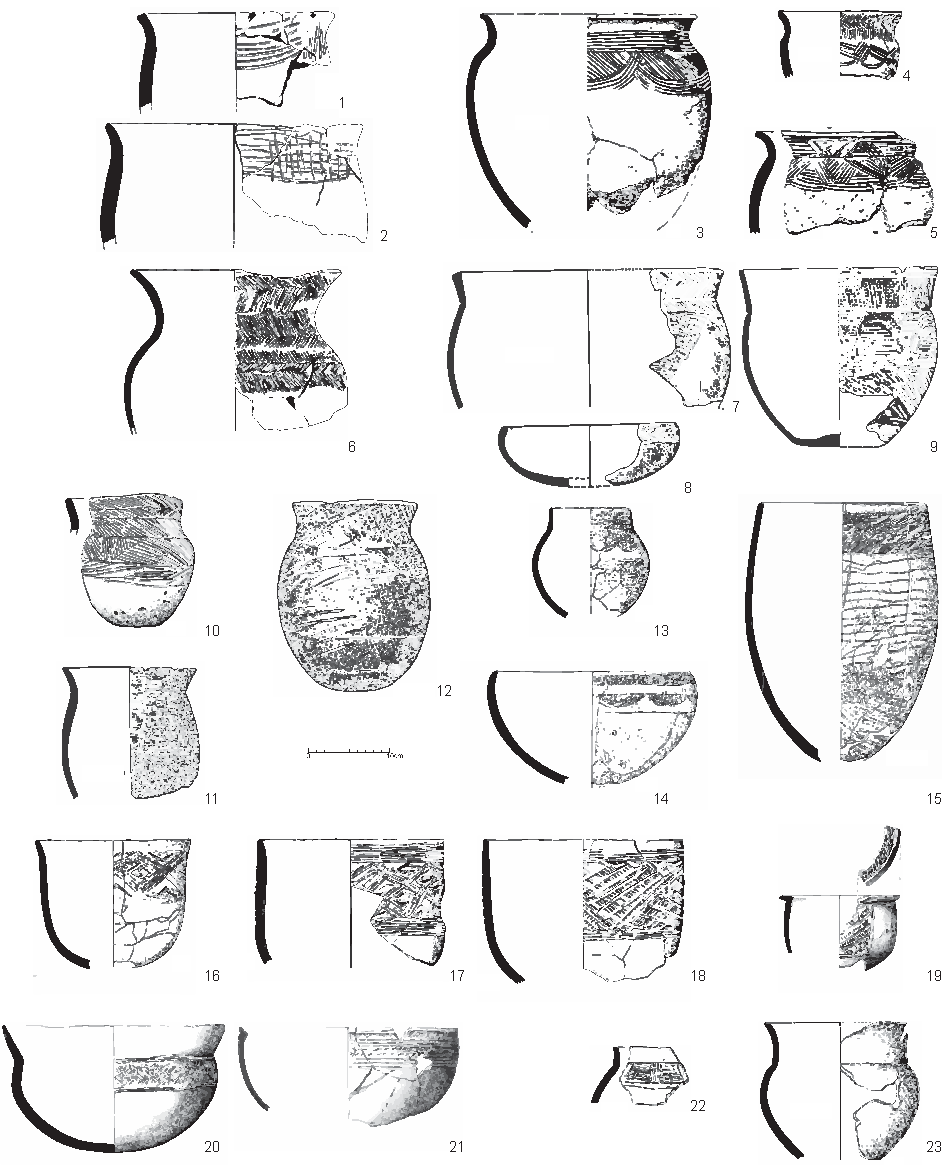
\includegraphics[width = \textwidth]{fig/Niederkongo_Typen.pdf}
	\caption{Niederkongo: Regionale Sequenz nach \textcites{deMaret.1982c}{deMaret.1986}{Gosselain.1988}{Denbow.2012}{Denbow.2014}.\\1--2: \textit{Ceramic Late Stone Age}, Phase 1 \parencite[148 Abb.~5]{Denbow.1990}; 3--5: Ngovo-Gruppe \parencite[108 Abb.~4.7, Abb.~4.11, 111 Abb.~5.3]{deMaret.1986}; 6: Herringbone-Gruppe \parencite[156 Abb.~10]{Denbow.1990}; 7--9: Kay~Ladio-Gruppe \parencite[454 Abb.~3.1--3]{Maret.1990}; 10--12: Gombe-Gruppe \parencites[Île des Mimosas; ][279 Abb.~8.1]{Eggert.1984}[454 Abb.~4.1--2]{Maret.1990}; 13--15: \textit{Groupe I} \parencite{deMaret.1972}; 16--18: \textit{Groupe II} \parencites{deMaret.1972}[Abb.~5.1--2]{Gosselain.1988}; 19: Kongo Typ B/\textit{Groupe V} \parencites{deMaret.1972}[Abb.~23.3]{vanNoten.1982}; 20: \textit{Groupe III} \parencites{deMaret.1972}[Abb.~23.1]{vanNoten.1982}; 21: Kongo Typ A/\textit{Groupe IV} \parencites{deMaret.1972}[Abb.~23.2]{vanNoten.1982}; 22--23: \textit{Groupe X} \parencite[483 Abb.~5.6]{deMaret.1999}.}
	\label{fig:Niederkongo_Sequence}
\end{figure*}

Zeugnisse, die auf die Produktion von Objekten aus Eisen hindeuten, sind ab dem 4.--2./1.~Jh. v.~Chr. entlang der Atlantikküste der Republik Kongo belegt \parencites[394]{Denbow.2012}[106--135]{Denbow.2014}.\footnote{Die frühesten Belege für die Nutzung von Eisen datieren in das 4.~Jh. v.~Chr. und stammen von der Fundstelle Lamba \parencite[394]{Denbow.2012}. Das spärliche Vorkommen von Zeugnissen von Eisenmetallurgie während der letzten Jahrhunderte v.~Chr. belegt für \textsc{Denbow} (ebd.) die Kontinuität zwischen den ins 13.--4.~Jh. v.~Chr. datierenden Inventaren aus Tchissanga-West und den Inventaren der Fundstellen Tchissanga-East, Mvindou sowie Lamba, die in das 4.--1.~Jh. v.~Chr. datieren.} Die keramischen Inventare der Fundstellen wandeln sich in dieser Zeit ebenfalls. Gefäße weisen nun runde Böden, umgelegte bis umgeschlagene, ausbiegende Ränder und prononcierte Schulterpartien auf \parencite[396\,f.]{Denbow.2012}. Verzierungen bestehen vornehmlich aus Kammeindrücken sowie Fischgrät-Mustern. Die einzelnen stilistischen Ausprägungen dieser Phase, namentlich die Gruppen \textit{Herringbone} (Abb.~\ref{fig:Niederkongo_Sequence}.6), \textit{Carinated Broadly Grooved} sowie \textit{Spaced Curvilinear}, werden von \textsc{Denbow} (ebd.) als individuelle \enquote{Waren} beschrieben und lassen sich bis in das 8.~Jh. n.~Chr. nachweisen.\footnote{Die entsprechenden Inventare weisen nur schwache stilistische Ähnlichkeiten zur zeitgleichen Keramik im nördlich angrenzenden Gabun auf, namentlich zu den Gruppen Oveng, Okanda sowie Otoumbi (\textsc{Denbow} 2014: 397; siehe Kap.~\ref{sec:Gabun}).} Am Ende dieser frühen Eisenzeit stehen Gefäße mit geraden Wandungen und breiter Riefenzier (ebd. 399\,f. Abb.~11), wie sie auch in Nordost-Angola gefunden wurden \parencite[201 No. 1--4, 7]{Clark.1968b}. Der Beginn der Späten Eisenzeit datiert nach \textcite[402--404]{Denbow.2012} ins 11.~Jh. n.~Chr., im Anschluss an eine etwa drei Jahrhunderte überspannende Lücke in der Sequenz der Loango-Küste. \textsc{Denbow} (ebd.) untergliedert diese Periode in einen frühere, bis an das Ende des 16.~Jh. n.~Chr. reichende Stufe, die keine Spuren europäischen Handelswaren aufweist, sowie eine jüngere, entsprechende Kontaktfunde aufweisende.

Südlich des Kongoflusses werden potenziell ältere, in das 15.~Jh. v.~Chr. datierende Funde von der Fundstelle Sakuzi diskutiert \parencites{deMaret.1982b}[634]{deMaret.2013}, während die frühesten hinreichend sicher belegten keramischen Zeugnisse der ins 4.~Jh. v.~Chr. bis 1.~Jh. n.~Chr. datierenden Ngovo-Gruppe zuzurechnen sind \parencite{deMaret.1986}.\footnote{Vor allem Inventare von Höhlenfundstellen aus der Region südlich des Kongo zwischen seiner Mündung in den Atlantik und dem Pool Malebo bilden den Grundstein des älteren Abschnitts der regionalen Sequenz. Surveyfunde aus Dibamba und Ngovo fanden Einzug in eine von Georges \textcites{Mortelmans.1962}{Mortelmans.1962b} zusammengestellte Sammlung \parencite[104]{deMaret.1986}. Dieser gliederte das keramische Material in sechs Gruppen (I--VI) und da keine stratigraphischen Relationen bekannt waren, ordnete er die einzelnen Gruppen entsprechend der Dicke ihrer mineralischen Verkrustung von \textit{alt} (Gruppe~I) nach \textit{jung} (Gruppe~VI). Eine Überarbeitung dieser Sammlung durch \textcites{deMaret.1972}{deMaret.1986} führte zu einer Umkehrung der von \textcites{Mortelmans.1962}{Mortelmans.1962b} postulierten Sequenz: die ursprünglich als jüngste angesehen Keramik der Gruppe VI stellte sich als die älteste keramische Entwicklung der Region heraus und wurde von \textcite[104\,f.]{deMaret.1986} nach dem eponymen Fundort Ngovo benannt. Funde der Ngovo-Gruppe fanden sich auch in Kongo dia Vanga, wo sie mit geschliffenen Steinwerkzeugen assoziiert sind. Auch erste, in den Jahren 1972--73 durchgeführte Grabungen bestätigten die Stellung der Ngovo-Gruppe am Anfang der regionalen Sequenz des Niederkongo.} Die Ngovo-Keramik zeichnet sich durch flache Böden, dicke Wandungen und eine girlandenartige Ritzverzierung aus (ebd. 105; Abb.~\ref{fig:Niederkongo_Sequence}.3--5). Fünf Radiokohlenstoffdatierungen belegen die Stellung der Ngovo-Keramik am Beginn der regionalen Sequenz des Niederkongo.\footnote{Formale Entsprechungen findet die Ngovo-Keramik innerhalb des ebenfalls ins 2.~Jh. v.~Chr.--3.~Jh. n.~Chr. datierenden <Inventars der Grube am Flusskilometer 186 am \mbox{Likwala}-\mbox{aux}-\mbox{Herbes} (Kat.-Nr.~19; siehe Kap.~\ref{sec:SHG-LKW_Einzelfunde}; Abb.~\ref{fig:Ngovo_Typvertreter}).} Das Formenspektrum der jüngeren Kay Ladio-Gruppe, die sich auch nördlich des Kongo findet \parencite[83, 90]{Clist.1982}, leitet sich aus der vorhergehenden Ngovo-Keramik ab \parencites[60\,f.]{deMaret.1972}[125]{deMaret.1986}. Die frühesten Nachweise von Eisenmetallurgie, an der Fundstelle Sakuzi, sind mit Kay Ladio-Keramik vergesellschaftet und können auf Basis von zwei Radiokohlenstoffdatierungen (Lv-1468, Lv-1469) in das 1--4.~Jh. n.~Chr. datiert werden. Eine detaillierte Beschreibung der formalen Eigenschaften der Kay Ladio-Keramik liegt bislang nicht vor. \textcite[119 Abb.~10.10]{deMaret.1986} weist lediglich auf flächige Ritzverzierung hin, welche Kay Ladio und Ngovo-Keramik unterscheiden (Abb.~\ref{fig:Niederkongo_Sequence}.7--9).\footnote{Durch neuere Feldarbeiten im Zuge des KongoKing-Projektes (siehe Anm.~\ref{ftn:KongoKingProj}) wurde eine Kitala-Gruppe erfasst, die in das 3.--4.~Jh n.~Chr. datiert \parencite{Clist.2019a}. Die Kitala-Keramik entspricht zeitlich der jüngeren Phase der Kay Ladio-Gruppe und ist bislang nur an wenigen Fundplätzen südlich des Kongo-Flusses belegt.}

Weder Ngovo- noch Kay Ladio-Keramik ist weiter den Kongo stromauf, im Gebiet des Pool Malebo belegt. Die bislang älteste beschriebene Keramik aus dieser Region stammt von der Fundstelle Gombe in Kinshasa (ebd. 127).\footnote{Die Steinartefakte der Fundstelle Pointe de Gombe (ehem. Pointe Kalina) in Kinshasa wurden von \textcites{Colette.1933}{Colette.1935}[81\,f.]{Bequaert.1938} einem \textit{Néolithique léopoldien} zugewiesen. \textcites{Mortelmans.1962b} griff diese Konzeption auf und erweiterte sie um die geschliffenen Steingeräte des Niederkongo.} Die in Gombe gefundene Keramik lässt sich zweifelsfrei mit Zeugnissen von Eisenmetallurgie assoziieren. Leider lassen sich aufgrund umfangreicher Störungen an Fundstellen keine genaueren Angaben machen \parencites{Cahen.1976}{deMaret.1999}. Drei Thermolumineszenzdatierungen aus Gombe legen eine Datierung zwischen das 3.--5.~Jh. n.~Chr. nahe \parencite[131]{Cahen.1981}. Typologisch sieht \textcite[130]{deMaret.1986} deutliche Ähnlichkeiten zwischen der Keramik aus Gombe (Abb.~\ref{fig:Niederkongo_Sequence}.10--12) und der Ngovo-Gruppe: beide Gruppen zeichnen sich durch flache Böden und morphologisch relativ einfache Gefäße sowie eine technisch eher grob ausgeführte Verzierung im Schulter- und Halsbereich aus. Ebenfalls der Gombe-Gruppe zuzuordnen sind 27 von H. Van~Morsel gesammelte, bisher nicht umfassend vorgelegte Gefäße von der Île des Mimosas \parencites[79]{deMaret.1982c}[279\,f. Abb.~8--9]{Eggert.1984}.\footnote{In den 1980er Jahren wurde die Keramik von der Île des Mimosas von Manfred K.~H. Eggert im \textit{Musée du Campus de l'Université de Kinshasa} fotografiert und umgezeichnet sowie teilweise veröffentlicht (\textsc{Eggert} 1984: 279--280 Abb. 8--9). Die bislang einzigen Belege für Schamott-Magerung, bestimmendes Merkmal der ausschließlich im äußersten Süden des Arbeitsgebietes verbreiteten Bobusa-Keramik (Kap.~\ref{sec:BBS-Gr}), stammen aus dem Gebiet des Pool Malebo \parencites[585--587]{Cahen.1976} sowie dem Niederkongo \parencites{Gosselain.1988}[118]{Denbow.2014} und umfassen auch die Gefäße von der Île des Mimosas. Siehe auch Anm.~\ref{ftn:IleMimosas}.}

Der jüngere Teil der regionalen Sequenz wurde zwischen 2012 und 2017 durch das KongoKing-Projekt\footnote{Der archäologische Teil des interdisziplinären KongoKing-Projektes war vornehmlich der Erforschung der Entwicklung des Kongo-Königreiches gewidmet. Zudem wurden die Einflüsse des ersten europäischen Kontaktes auf die Region untersucht.\label{ftn:KongoKingProj}} einer grundsätzlichen Neubewertung unterzogen \parencites[443 Abb.~31.1]{Clist.2018b}{Clist.2018c}. Die ab dem 13.~Jh. n.~Chr. belegte Kindoki-Gruppe markiert den Beginn des jüngeren Abschnitts der Sequenz im Niederkongo (ebd. 245--253). Kennzeichen der Kindoki-Keramik sind horizontale Bänder aus diagonal gestellten Kammeindrücken auf der Gefäßschulter (ebd. 245 Abb.~19.4, 247 Abb.~19.5). Die Mbafu-Gruppe umfasst jene charakteristischen Schalen-Formen, die von \textcites{Mortelmans.1962}{Mortelmans.1962b} der \textit{Groupe~II} genannten Phase zugerechnet wurden (Abb.~\ref{fig:Niederkongo_Sequence}.16--18). Von \textcite[193\,f.]{Clist.2012a} wird eine Untergliederung in zwei Fazies vorgeschlagen, die von \textcite{Cranshof.2018} zu zwei Stilgruppen ausgearbeitet werden.\footnote{Siehe auch \textcite[249 Tab.~19.1]{Clist.2018c} für eine tabellarische Übersicht der Gemeinsamkeiten und Unterschiede der beiden Stile beziehungsweise Fazies des ehemals als \textit{Groupe~II} beschriebenen Materials.} Der Dimba-Stil\footnote{Der Dimba-Stil entspricht der von \textcite[193\,f.]{Clist.2012a} vorgeschlagenen Mbafu-Fazies; er wurde von \textcite{Cranshof.2018} umbenannt, um eine einheitliche Nomenklatur zu schaffen.} (ebd. 178--182 Abb.~7.4) umfasst vor allem das von \textcites{Mortelmans.1962}{Mortelmans.1962b} gesammelte Inventar aus rundbodigen Schalen mit gerader Wandung und einer aufwendigen Verzierung aus sich diagonal überlagernden Ritzungen, die starke Ähnlichkeiten zu aus Raffia gewobenen Textilien sowie Korbflechtungen während der Zeit den Kongo-Königreiches aufweisen \parencite[170--176]{Cranshof.2018}. Die Datierungslage für den Dimba-Stil ist nicht zufriedenstellend und erlaubt lediglich eine grobe Einordnung in die zweite Hälfte des 15.~Jh. bis ins frühe 19.~Jh. n.~Chr. (ebd. 181). Die zweite Fazies der Mbafu-Gruppe (ehem. \textit{Groupe~II}) ist der Misenga-Stil, dem neben Schalenformen auch ein größeres Inventar aus geschlossenen Formen zugerechnet sind (ebd. 182--184 Abb.~7.5). Die chronologische Stellung des Misenga-Stils lässt sich auf das 14.--15.~Jh. n.~Chr. eingrenzen (ebd. 184).\footnote{Von \textcite{Denbow.2014} wird für die Atlantikküste der Republik Kongo unter der Bezeichnung \textit{Woven Ware} ebenfalls eine Keramik beschrieben, deren Verzierung an gewebte Motive erinnert und die aus zwei Stilgruppen besteht. Während der ältere Stil in Grabungen erfasst wurde und in das 12.--15.~Jh. n.~Chr. datiert werden kann, lässt sich der zweite, nur aus Oberflächenabsammlungen bekannte Stil, lediglich aufgrund der mit ihm vergesellschafteten europäischen Kontaktfunde in einen Zeitraum ab dem 16.~Jh. n.~Chr. einordnen \parencite[ebd. 69\,f., 136;][188\,f.]{Cranshof.2018}.}

Ab dem 15.~Jh. n.~Chr. setzt eine höhere Standardisierung der Töpfereierzeugnisse ein \parencite[444]{Clist.2018b}, die direkt mit dem Kongo-Königreich\footnote{Der Erstkontakt mit Europäern erfolgte 1483, als Portugiesen unter dem Kommando von Diogo C\~ao die Mündung des Kongo-Flusses und die Hauptstadt Mbanza Kongo erreichten \parencites[89]{Thornton.2001}[443\,f. Abb.31.1]{Clist.2018b}.} in Verbindung zu bringen ist und von \textcite[254--275]{Clist.2018c} in vier Untergruppen (A--D) unterteilt wird.\footnote{Die Untergliederung basiert auf der unveröffentlichten Auswertung der Keramik aus der Grabung von 1936 in Ngongo Mbata durch G.~Schellings und  M.~Bequaert \parencites{Vandenhoute.1973}[76]{Clist.2018d} und der Feldarbeit des KongoKing-Projektes zwischen 2012--2015.} Typ~A besteht aus rundbauchigen und -bodigen Schalen mit auffällig gerillter Randlippe (ebd. 255\,f. Abb.~19.12--14) und datiert in das \mbox{15.--18.~Jh.} n.~Chr. (ebd. 257\,f. Tab.~19.3).\footnote{In Mbanza Kongo ist Keramik des Typs~A über das 15.--17.~Jh. n.~Chr. hinweg belegt (\textsc{Clist} u.~a. 2018c: 257) und fünf mit Keramik des Typs~A assoziierte Radiokohlenstoffdatierungen aus Kindoki decken ebenfalls das 15.--17.~Jh. n.~Chr. ab (ebd. 257\,f. Tab. 19.3). Die Grabungen in Ngongo Mbata deuten auf ein Bestehen des Typs~A bis in das 18.~Jh. n.~Chr. hin (ebd. 258). Die Schalen des Typs~A zeigen auffällige Ähnlichkeiten zu jenen Formen, die von \textcites{Mortelmans.1962}{Mortelmans.1962b} der \textit{Groupe~IV} zugerechnet wurden \parencite[258 Abb.~19.16; Abb.~\ref{fig:Niederkongo_Sequence}.21]{Clist.2018c}.} Die Keramik des Typs B ist durch leicht gebauchte, häufig kleine Gefäße mit auffällig umgeschlagenen Rändern gekennzeichnet. Die Ornamentik besteht vor allem aus horizontalem oder wellenförmigem Kammstrich sowie ritzgefüllten Rauten und findet sich ausschließlich auf dem oberen Teil der Wandungen (ebd. 260 Abb.~19.17). Der Typ~B entspricht dem von \textcites{Mortelmans.1962}{Mortelmans.1962b} als \textit{Groupe~V} beschriebenen Material (Abb.~\ref{fig:Niederkongo_Sequence}.19).\footnote{Von \textcite[23]{Gosselain.1988} werden Parallelen der \textit{Groupe~V}-Keramik  (Abb.~\ref{fig:Niederkongo_Sequence}.19), die seinerzeit lediglich aus Dimba und Mbanza Mbata belegt war, zu den Schalen der \textit{Groupe~II} (Abb.~\ref{fig:Niederkongo_Sequence}.16--18) diskutiert.} Die chronologische Position der Inventare kann auf das späte 16.--18.~Jh. n.~Chr. eingegrenzt werden \parencite[261]{Clist.2018c}. Der Typ~C ist durch Gefäße mit Kegelhals und ausbiegendem Rand, welcher innenseitig regelhaft einen scharfen Umbruch aufweist, gekennzeichnet. Die Verzierung der Keramik des Typs~C besteht aus Kombinationen von Ritzlinien und Rillen, häufig sich überkreuzend oder in Winkeln, jedoch immer durch horizontale Rillen eingefasst, die sich auf den Schulter- beziehungsweise Halsbereich der Gefäße beschränken (ebd. Abb.~19.20).\footnote{Die Keramik des Typs~C erinnert grob an die von \textcites{Mortelmans.1962}{Mortelmans.1962b} beschriebene \textit{Groupe~III} (Abb.~\ref{fig:Niederkongo_Sequence}.20). Die Schalen mit geschweifter Wandung und runden Böden dieser Gruppe lassen sich auf Basis einer Radiokohlenstoffdatierung aus Kamuna in das 15. bis frühe 17.~Jh. n.~Chr. datieren \parencites[82]{deMaret.1982c}[20]{Gosselain.1988}. Derselbe Befund enthielt auch Keramik der \textit{Groupe~II} nach \textcites{Mortelmans.1962}{Mortelmans.1962b}.} Der Typ~C ist für die gesamte in Kindoki und Ngongo Mbata erfasste Sequenz belegt und lässt sich folglich zwischen das 16.--18.~Jh. n.~Chr. datierten (ebd. 266). Eine Gruppe sehr aufwendig verzierter, jedoch stark fragmentierter Scherben, die bislang ausschließlich in Mbanza Kongo, Ngongo Mbata und Kindoki erfasst wurde, wird als Typ~D subsumiert beschrieben \parencite[267--274]{Clist.2018c}.\footnote{\textcite[184--187 Abb.~6.7]{Cranshof.2018} führen die entsprechenden Formen als \enquote{D-Pots}.} Diagnostisches Merkmal der Keramik des Typs~D ist eine aufwendige, in Ritztechnik erzeugte und in horizontalen Bändern oder Metopen organisierte Verzierung (ebd.~269--271). Die Ränder des Typs~D sind durchweg sehr kurz, verdickt und frei von Verzierungen (ebd.~268 Abb.~19.23--24, 270 Abb.~19.26). Die in das späte 16. bis frühe 18.~Jh. n.~Chr. datierende Keramik des Typs~D wurde lediglich bei den Grabungen in Mbanza Kongo, Ngongo Mbata und Kindoki erfasst (ebd. 184\,f., 187).

Für die von \textcites{Mortelmans.1962}{Mortelmans.1962b} der \textit{Groupe~I} zugewiesene Keramik liegen gegenwärtig keine Datierungsindizien vor. Die vornehmlich hohen Gefäßformen und die aus horizontalen Bändern bestehende, flächige Verzierung (Abb.~\ref{fig:Niederkongo_Sequence}.13--15) erinnert jedoch an Formen im östlichen Gabun, die \textcites[292 Taf.~21.2--3]{AssokoNdong.20002001}[147]{AssokoNdong.2002} als \textit{Okandéen} systematiert und in das 4. Jh. v.~Chr.--8.~Jh. n.~Chr. datiert. Für aus Kingabwa und Gombe stammende Keramik, die erstmals von \textcite[135]{Cahen.1981} beschrieben wurde, postuliert \textcite{deMaret.1982c} die Zuweisung zu einer neuen \textit{Groupe~X}. Eine Radiokohlenstoffdatierung aus Gombe (GrN-7218) stellt diese Keramik in das 18.--19.~Jh. n.~Chr. (ebd. 83). \textcite[22]{Gosselain.1988} ordnet der Gruppe~X noch eine weitere, in das 15.--18.~Jh. n.~Chr. fallende Datierung aus Kingabwa zu (Hv-6262), die \textcite[83]{deMaret.1982c} als für die Gruppe~II-Keramik repräsentativ ansah.\footnote{Eine weitere Untergliederung der \textit{Groupe~X} wurde von \textcite{Pincon.1988} vorgeschlagen. Siehe auch \textcite[212 Anm.~3]{Wotzka.1995}.}